\chapter{Additional objective-first results}\label{ob-1 additional}
\section{Additional mode coupler designs}
In this section, we present additional mode coupler designs based 
    on the objective-first strategy outlined in chapter~\ref{ob-1}.
A wide, high-index waveguide is used at both the input and output ports,
    and all permutations of couplers are fabricated among
    the first four propagating modes.
\begin{figure}[h!]
    \centering
    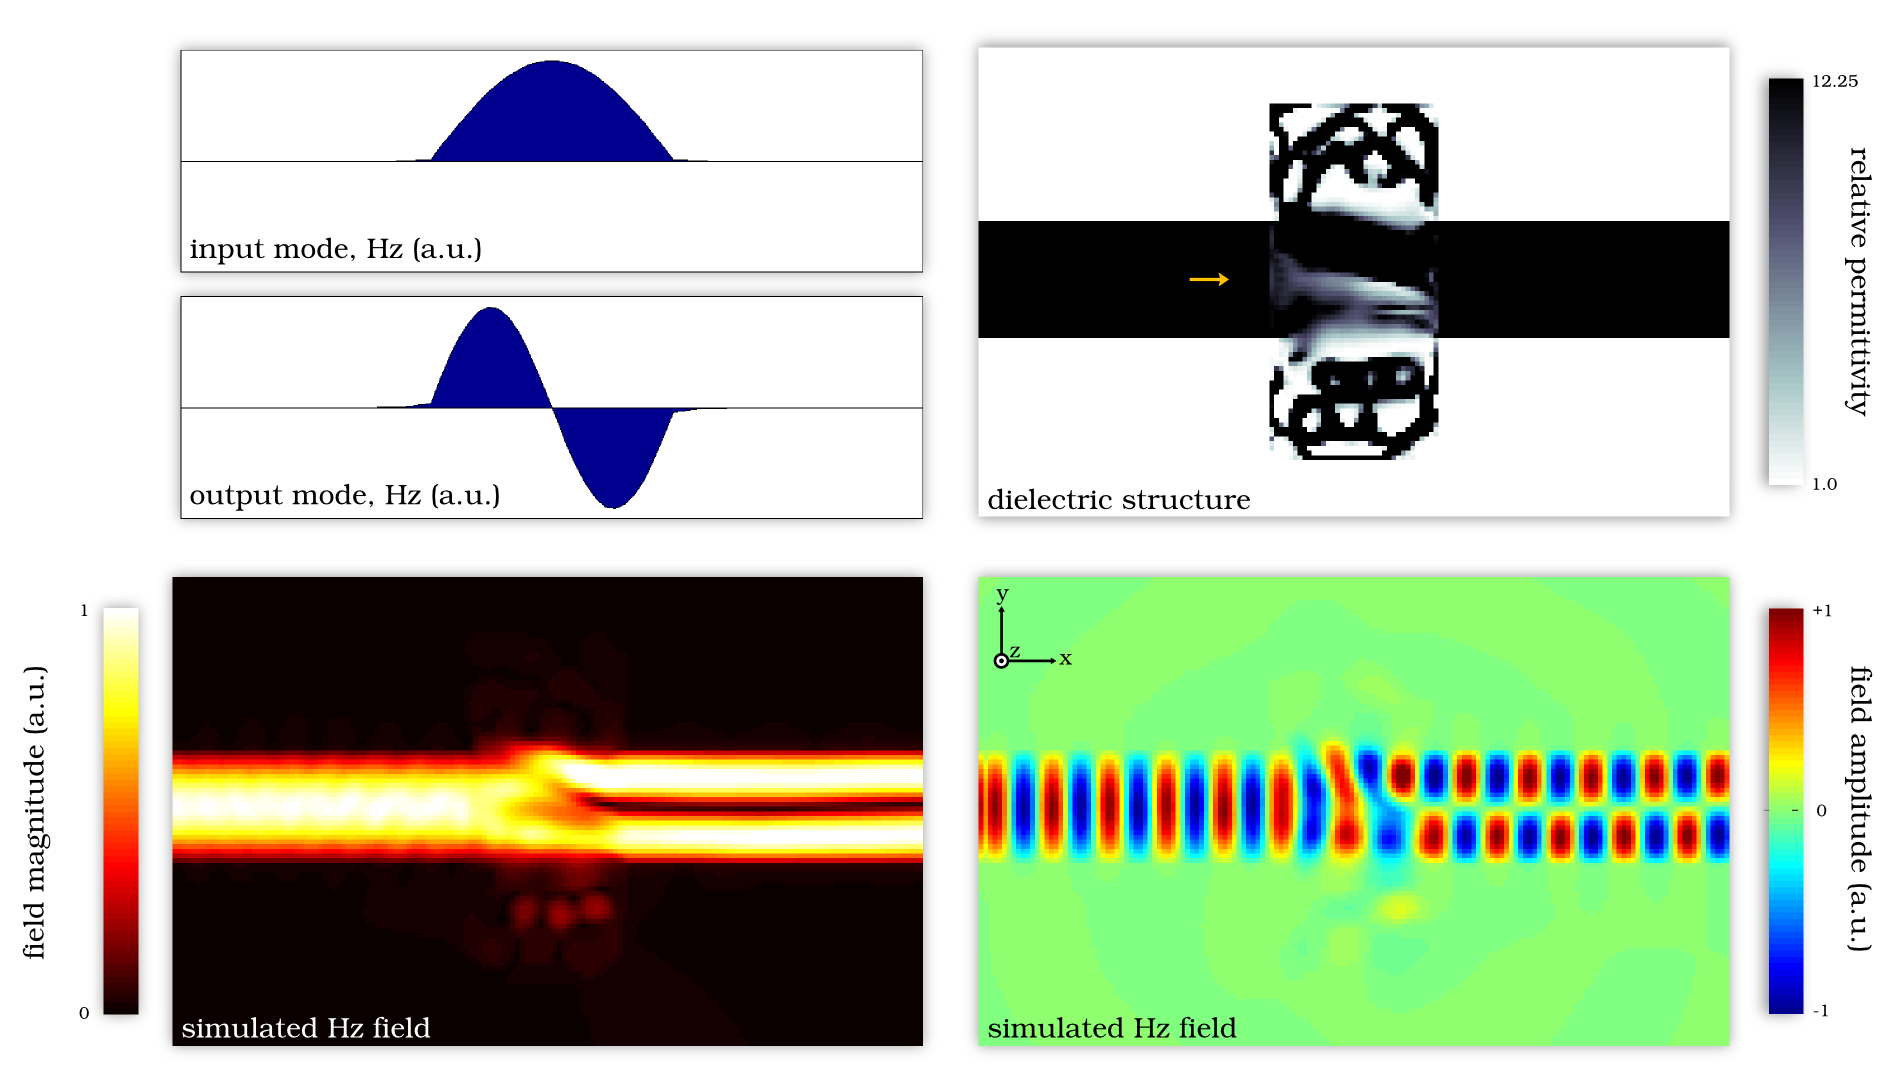
\includegraphics[width=\textwidth]{p3/6}
    \caption{
        Coupler from the first-order to the second-order mode 
            of a wide dielectric waveguide.
        Efficiency: $99.3\%$,
        footprint: $1.55$ square vacuum wavelengths.
        }
        % \label{fig:wire}
\end{figure}
\begin{figure}[h!]
    \centering
    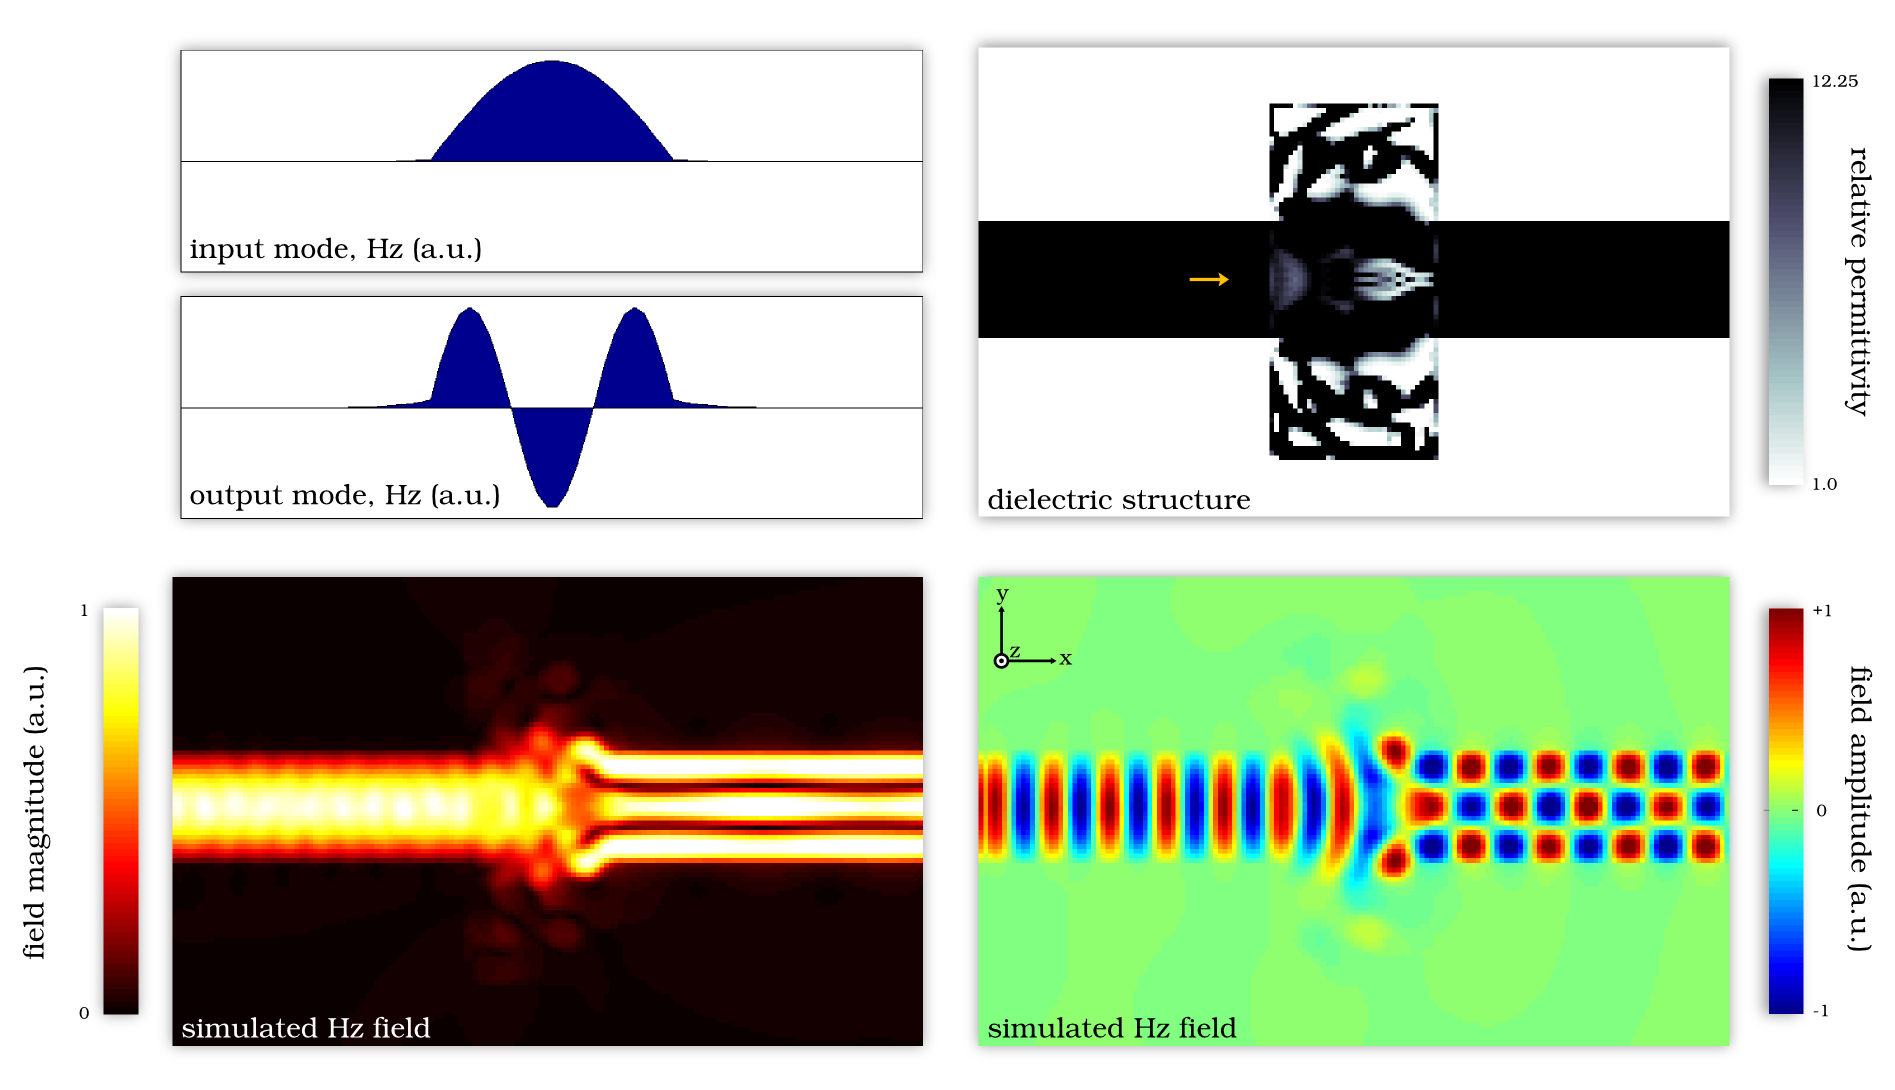
\includegraphics[width=\textwidth]{p3/7}
    \caption{
        Coupler from the first-order to the third-order mode 
            of a wide dielectric waveguide.
        Efficiency: $98.3\%$,
        footprint: $1.55$ square vacuum wavelengths.
        }
        % \label{fig:wire}
\end{figure}
\begin{figure}[h!]
    \centering
    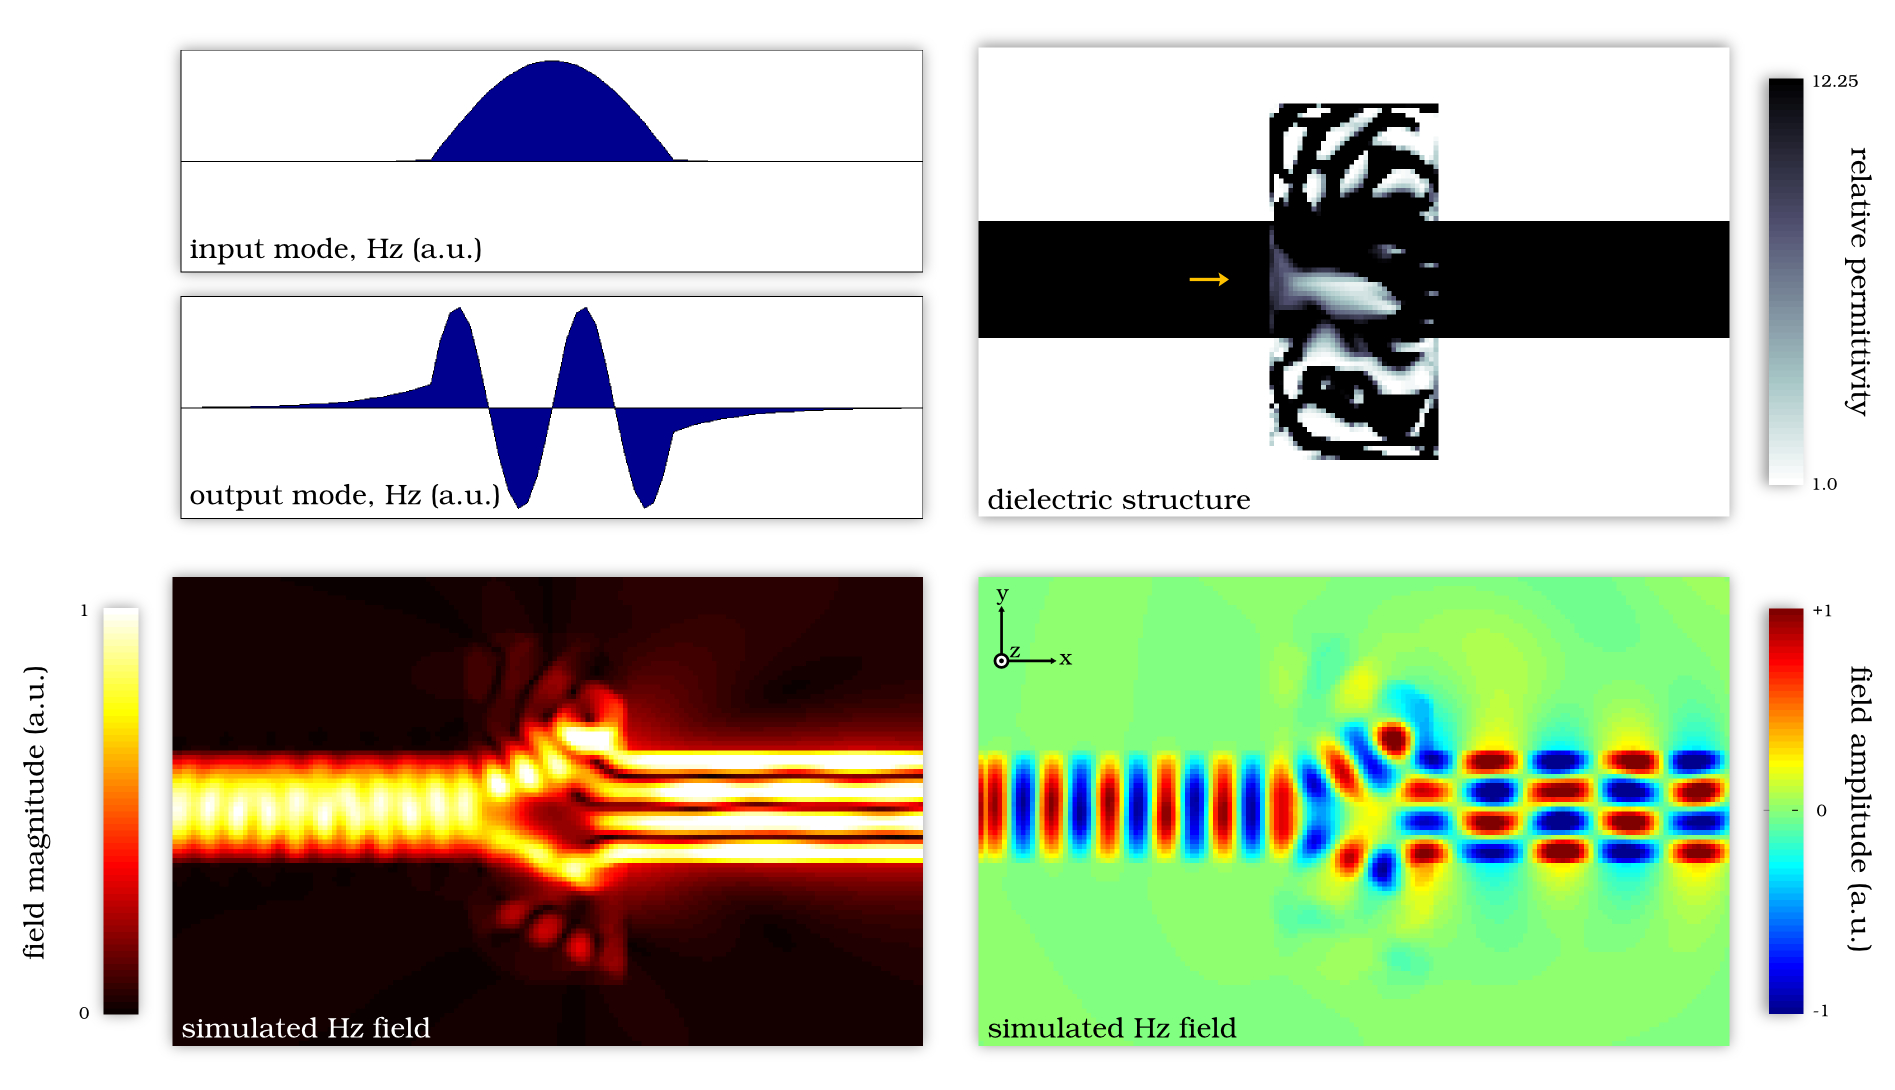
\includegraphics[width=\textwidth]{p3/8}
    \caption{
        Coupler from the first-order to the fourth-order mode 
            of a wide dielectric waveguide.
        Efficiency: $90.6\%$,
        footprint: $1.55$ square vacuum wavelengths.
        }
        % \label{fig:wire}
\end{figure}
\begin{figure}[h!]
    \centering
    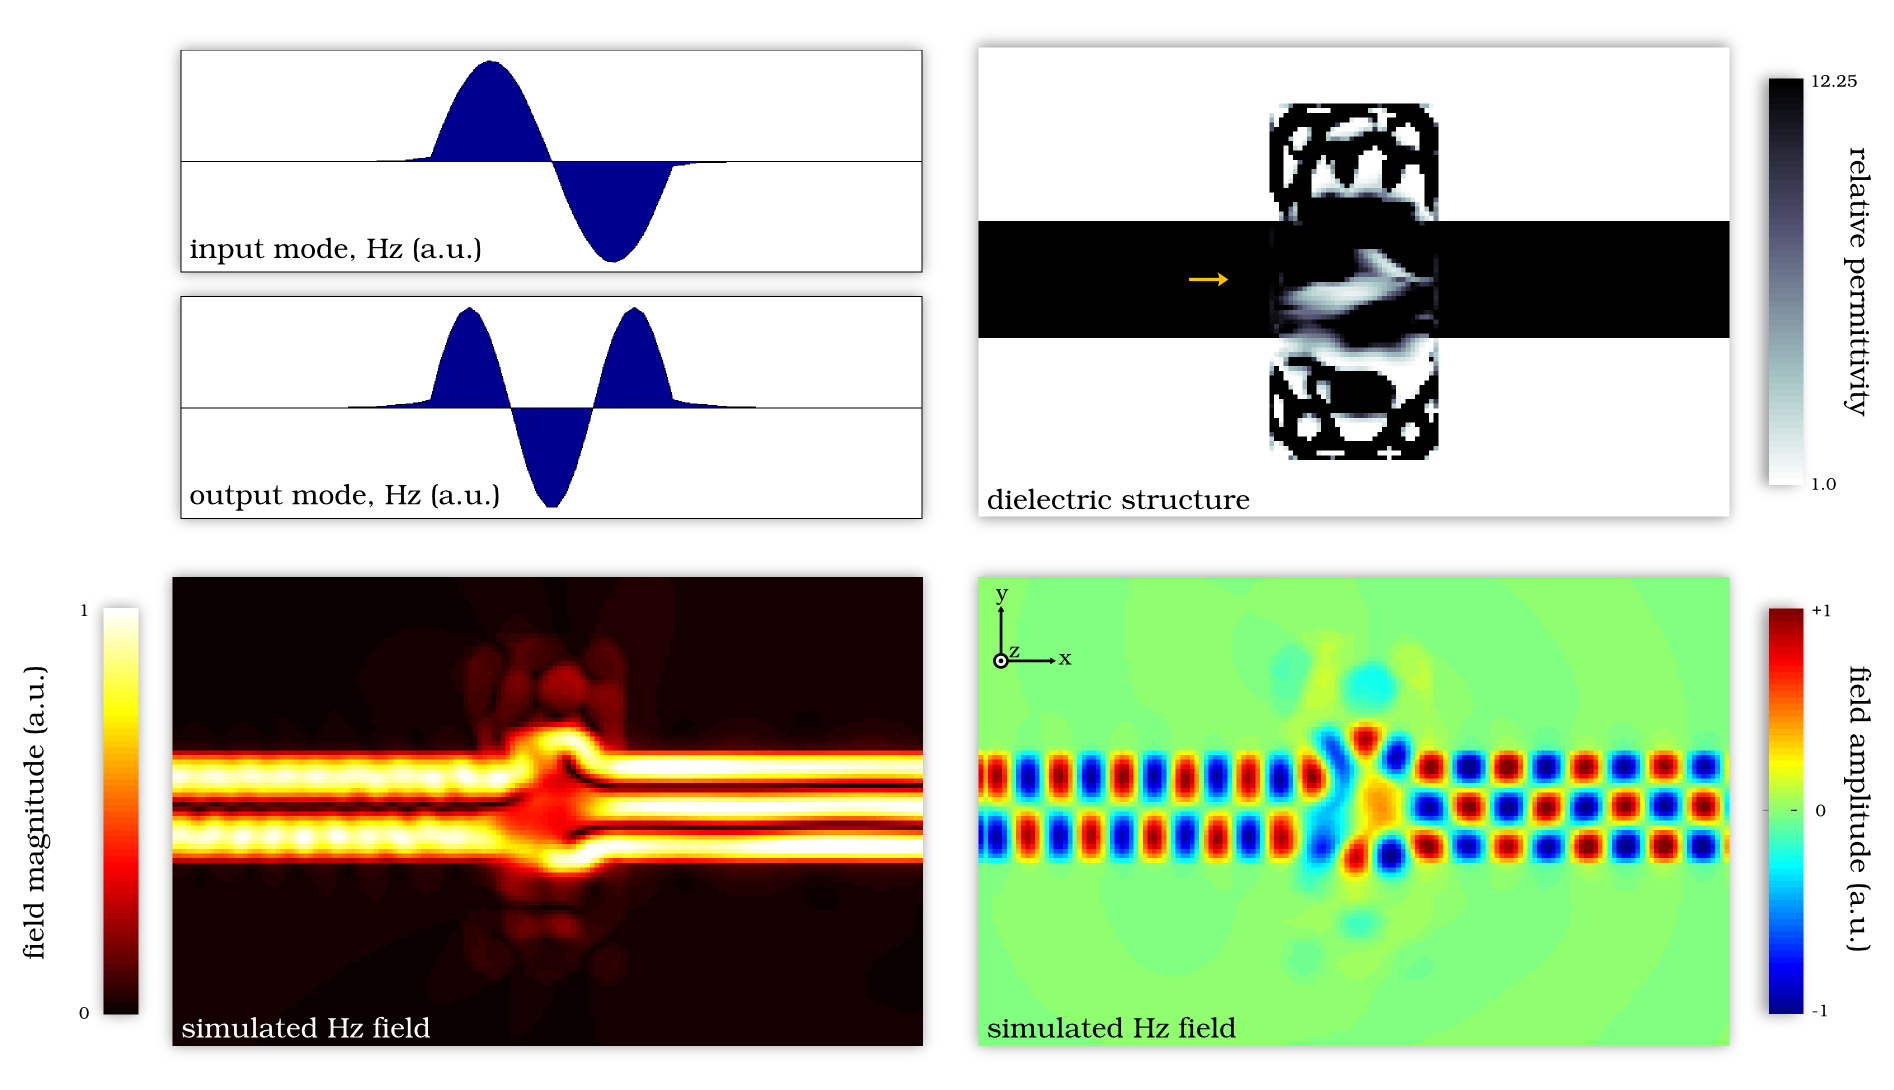
\includegraphics[width=\textwidth]{p3/9}
    \caption{
        Coupler from the second-order to the third-order mode 
            of a wide dielectric waveguide.
        Efficiency: $96.8\%$,
        footprint: $1.55$ square vacuum wavelengths.
        }
        % \label{fig:wire}
\end{figure}
\begin{figure}[h!]
    \centering
    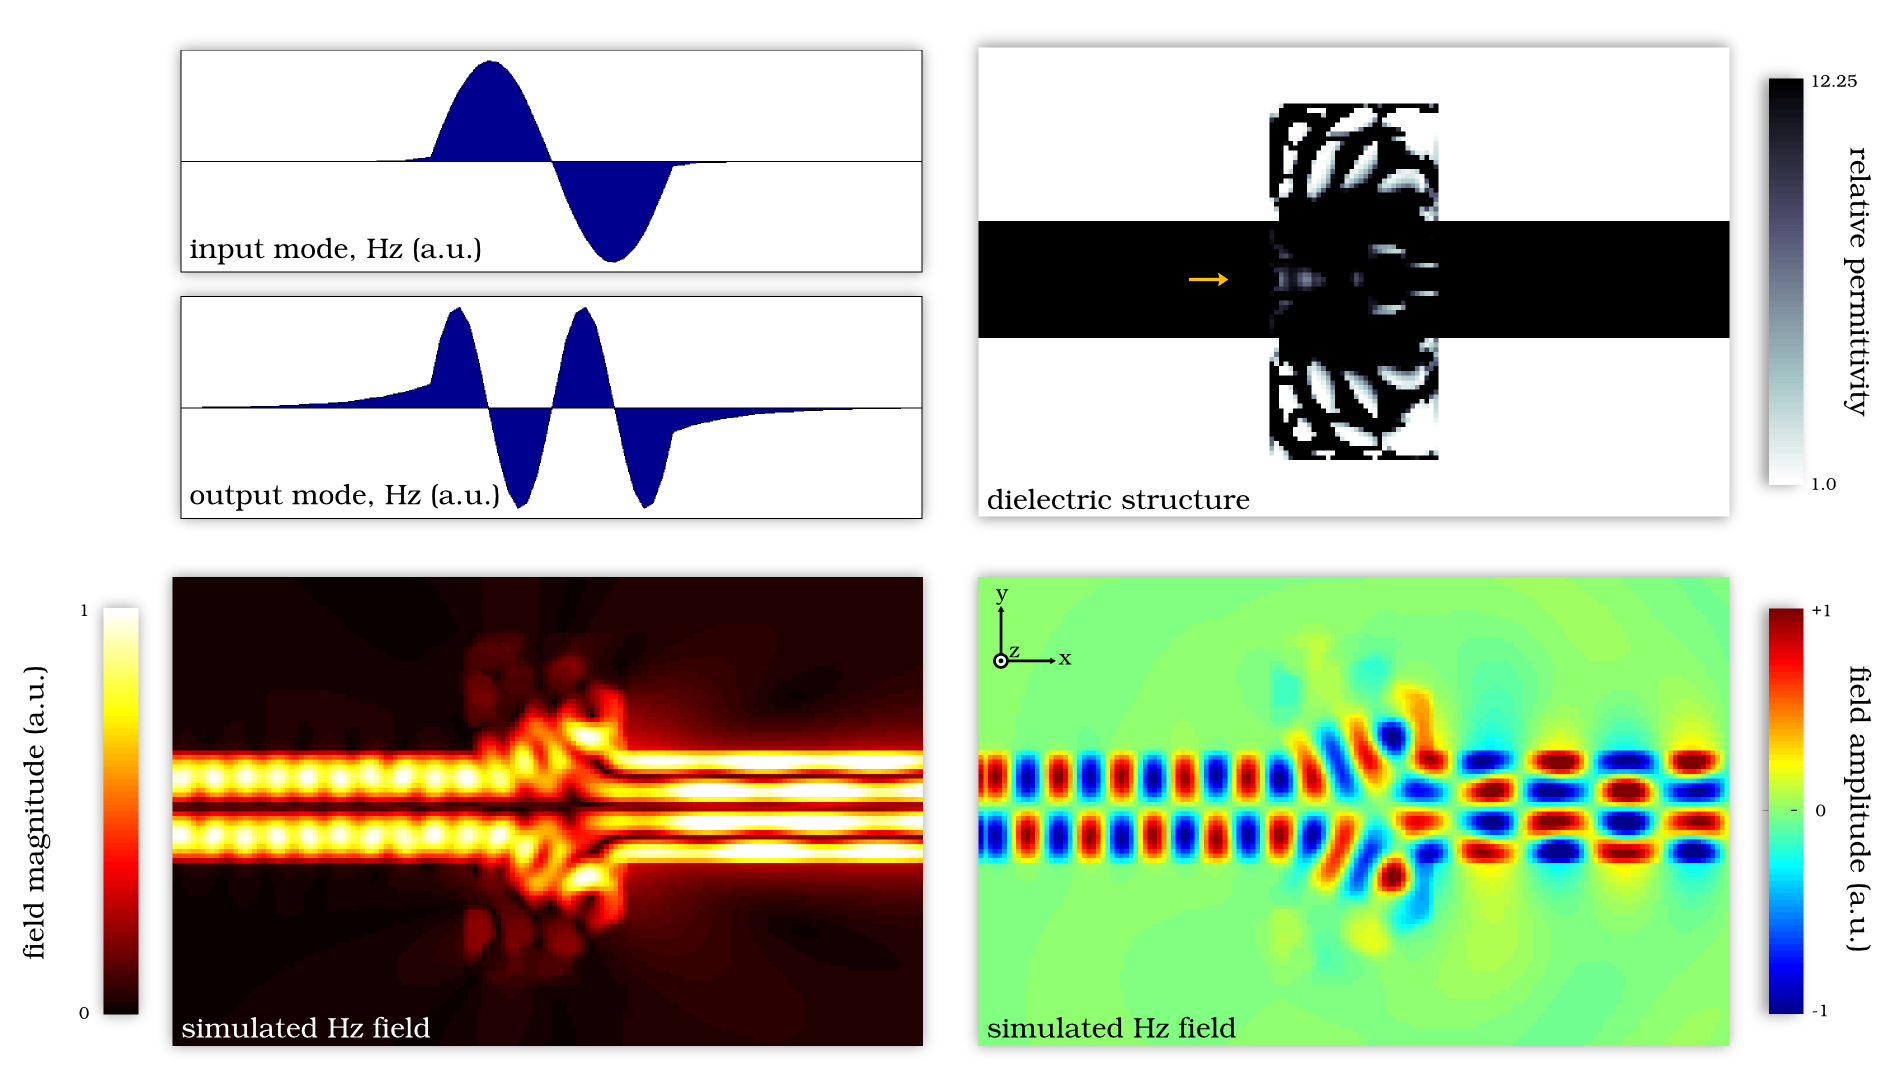
\includegraphics[width=\textwidth]{p3/10}
    \caption{
        Coupler from the second-order to the fourth-order mode 
            of a wide dielectric waveguide.
        Efficiency: $86.3\%$,
        footprint: $1.55$ square vacuum wavelengths.
        }
        % \label{fig:wire}
\end{figure}
\begin{figure}[h!]
    \centering
    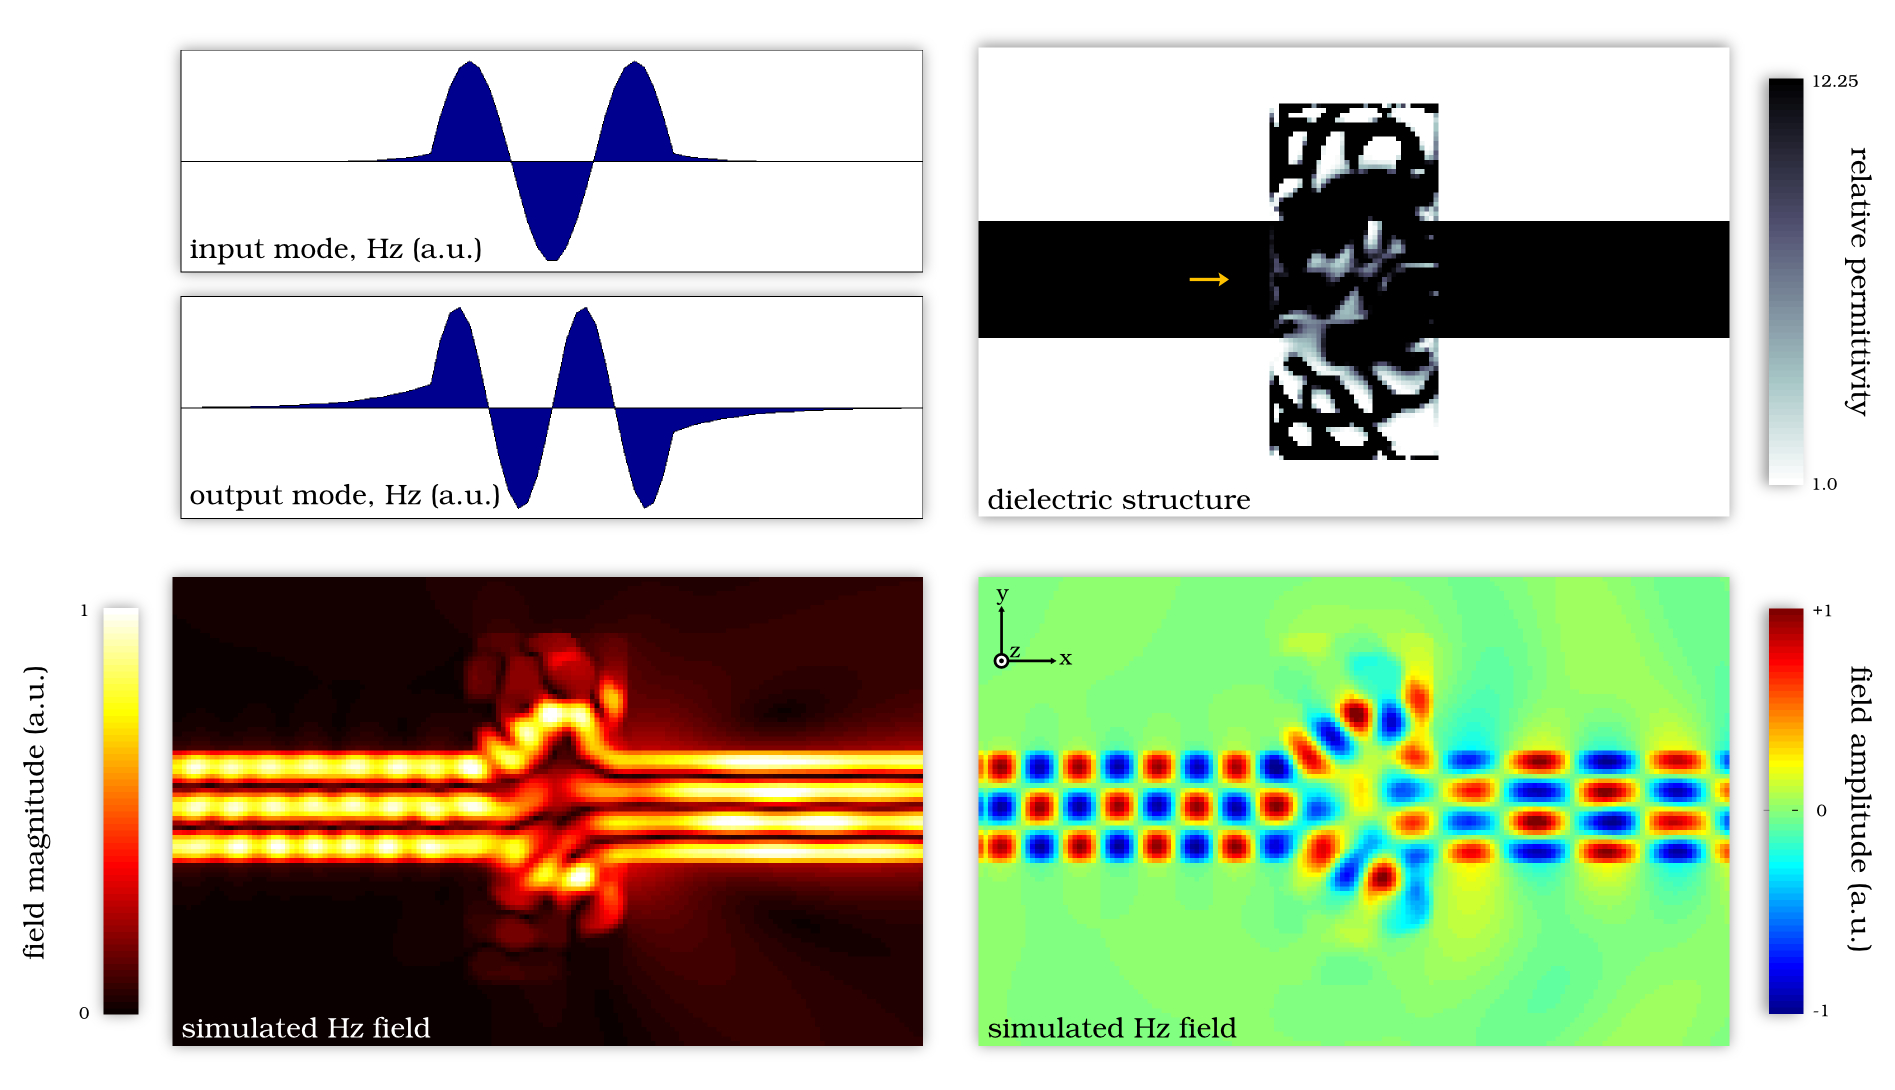
\includegraphics[width=\textwidth]{p3/11}
    \caption{
        Coupler from the third-order to the fourth-order mode 
            of a wide dielectric waveguide.
        Efficiency: $80.1\%$,
        footprint: $1.55$ square vacuum wavelengths.
        }
        % \label{fig:wire}
\end{figure}
\clearpage
\section{Additional designs with wide, low-index input waveguide}
We now reproduce Figs~\ref{fig:mode}-\ref{fig:wire}
    but instead use a wide, low-index waveguide as the input.
Once again, this is to demonstrate the generality of our method;
    namely, that it can be applied to the design of nearly any
    single-mode, linear nanophotonic device.
\begin{figure}[h!]
    \centering
    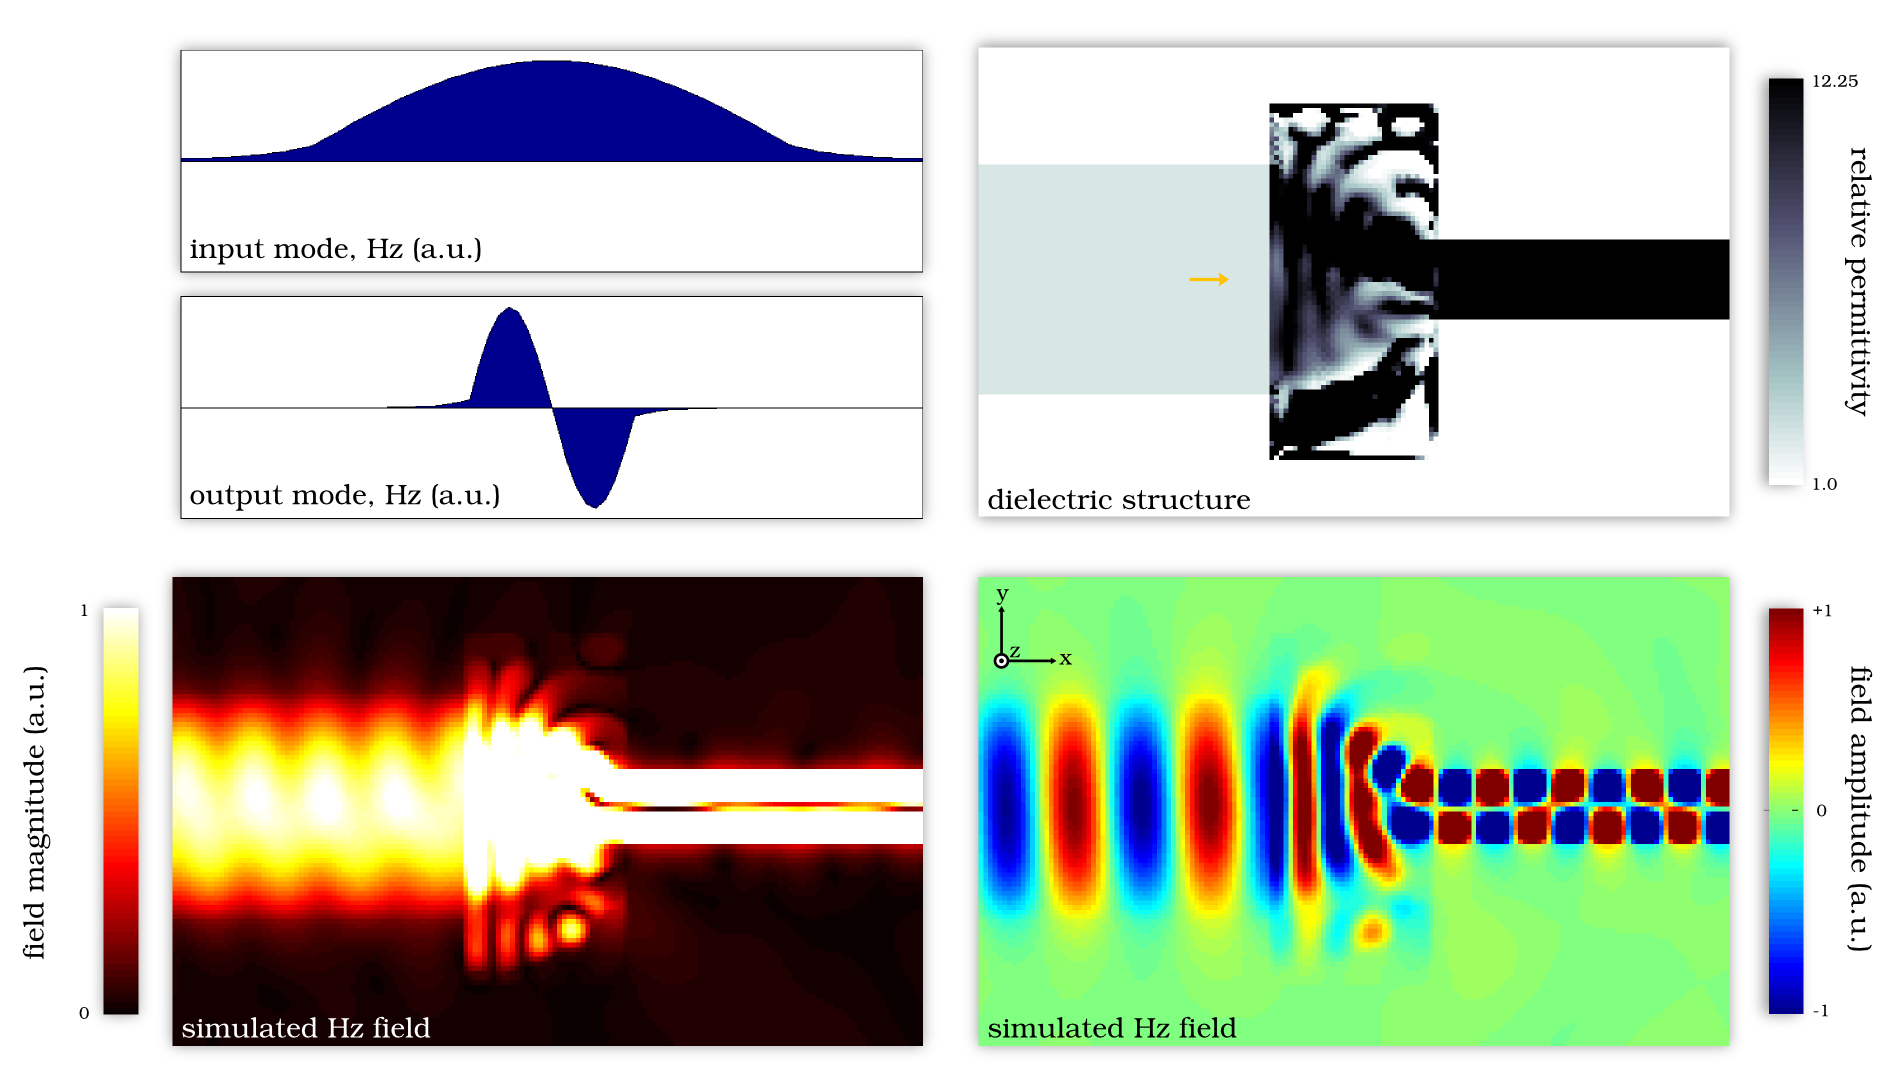
\includegraphics[width=\textwidth]{p3/12}
    \caption{
        Coupler from a wide, low-index waveguide to the
            second-order mode of a narrow, high-index waveguide.
        Efficiency: $96.9\%$,
        footprint: $1.55$ square vacuum wavelengths.
        }
        % \label{fig:wire}
\end{figure}
\begin{figure}[h!]
    \centering
    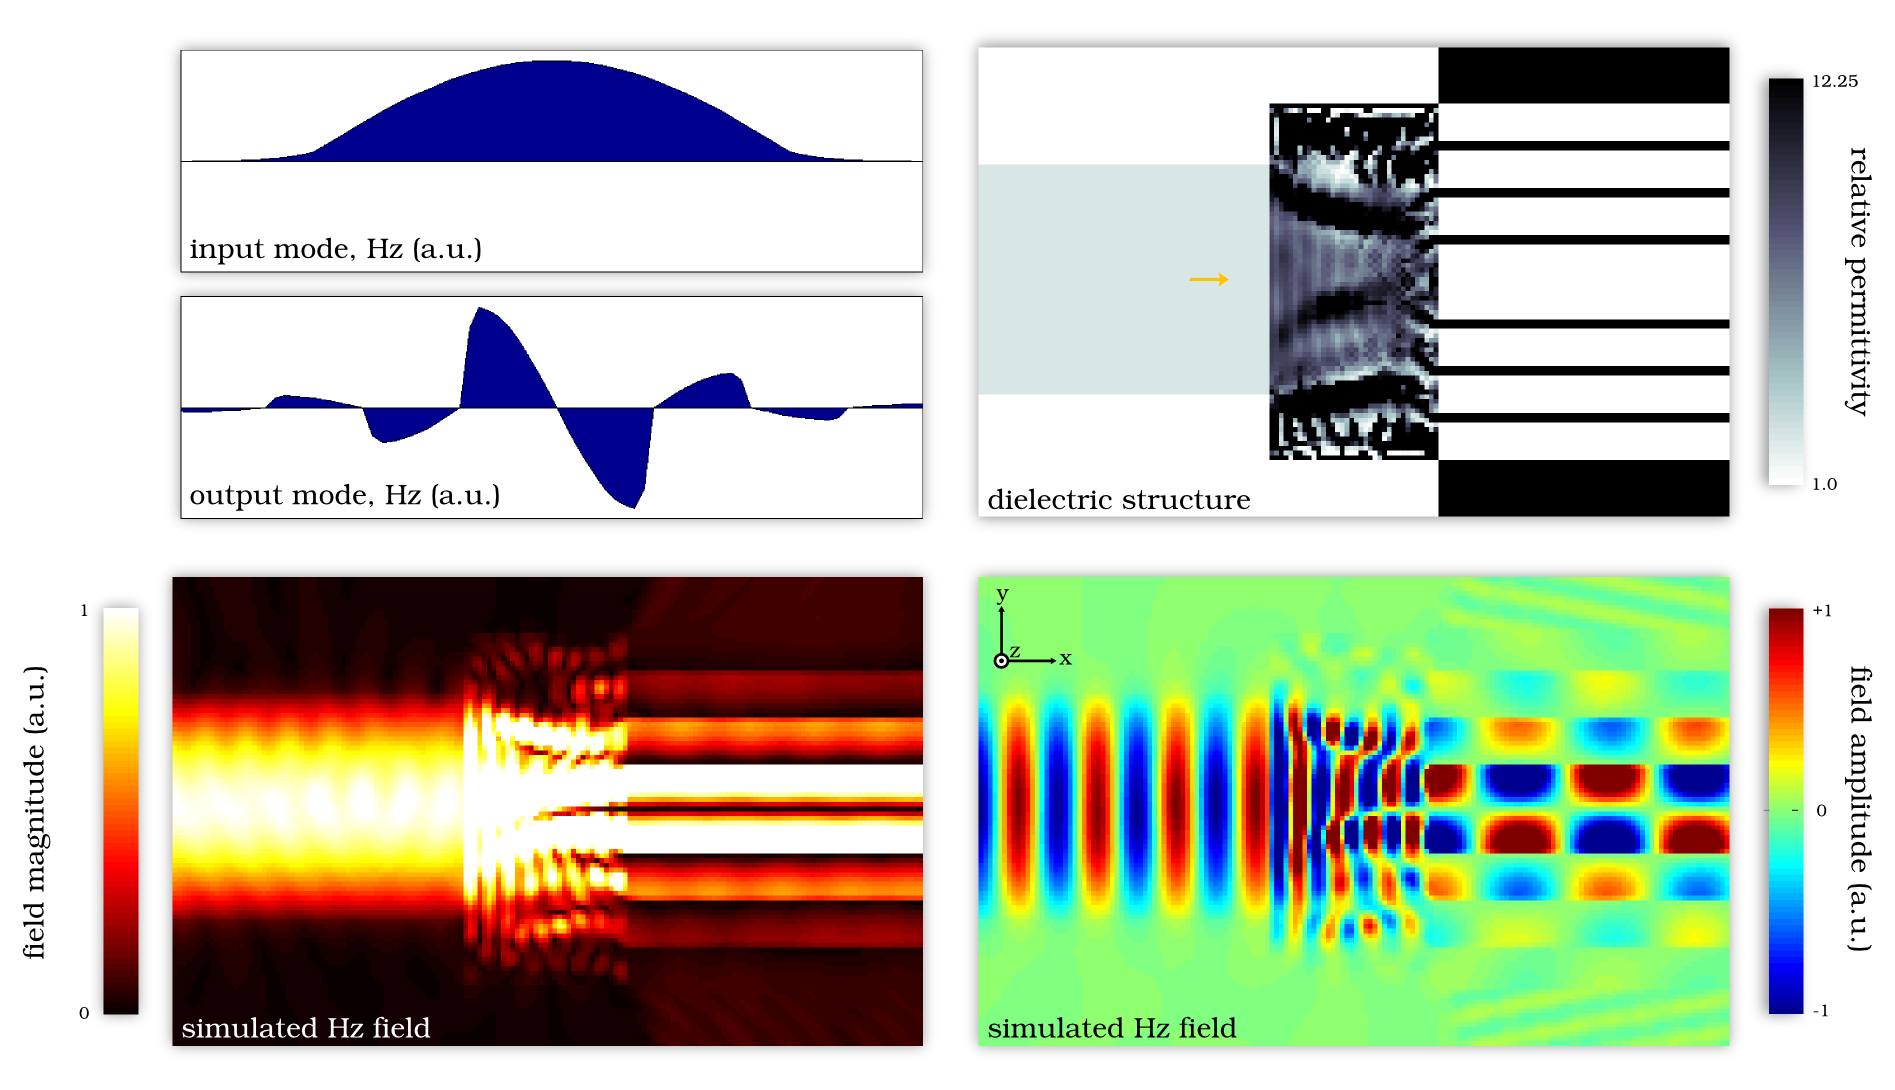
\includegraphics[width=\textwidth]{p3/13}
    \caption{
        Coupler from a wide, low-index waveguide to an 
            ``air-core'' waveguide mode.
        Efficiency: $99.0\%$,
        footprint: $4.38$ square vacuum wavelengths.
        }
        % \label{fig:wire}
\end{figure}
\begin{figure}[h!]
    \centering
    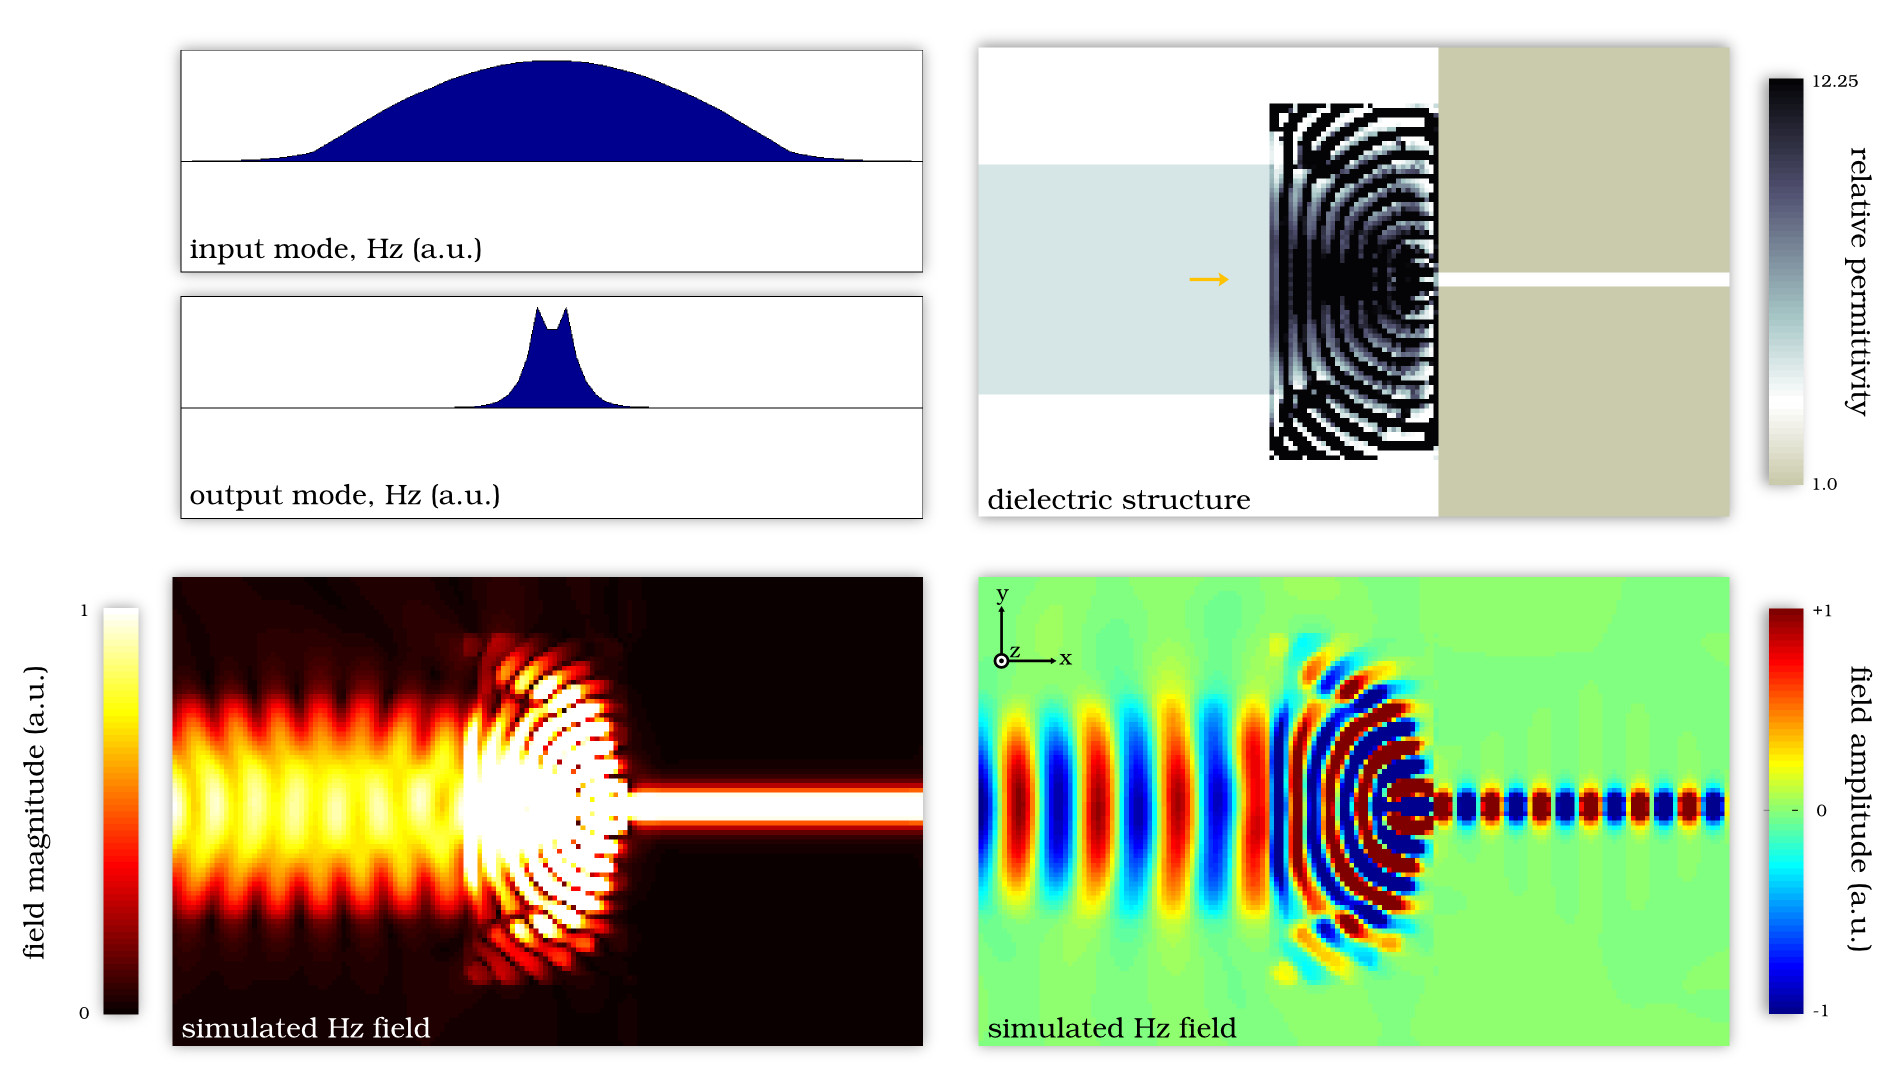
\includegraphics[width=\textwidth]{p3/14}
    \caption{
        Coupler from a wide, low-index waveguide to a
            metal-insulator-metal plasmonic waveguide mode.
        Efficiency: $96.7\%$,
        footprint: $4.38$ square vacuum wavelengths.
        }
        % \label{fig:wire}
\end{figure}
\begin{figure}[h!]
    \centering
    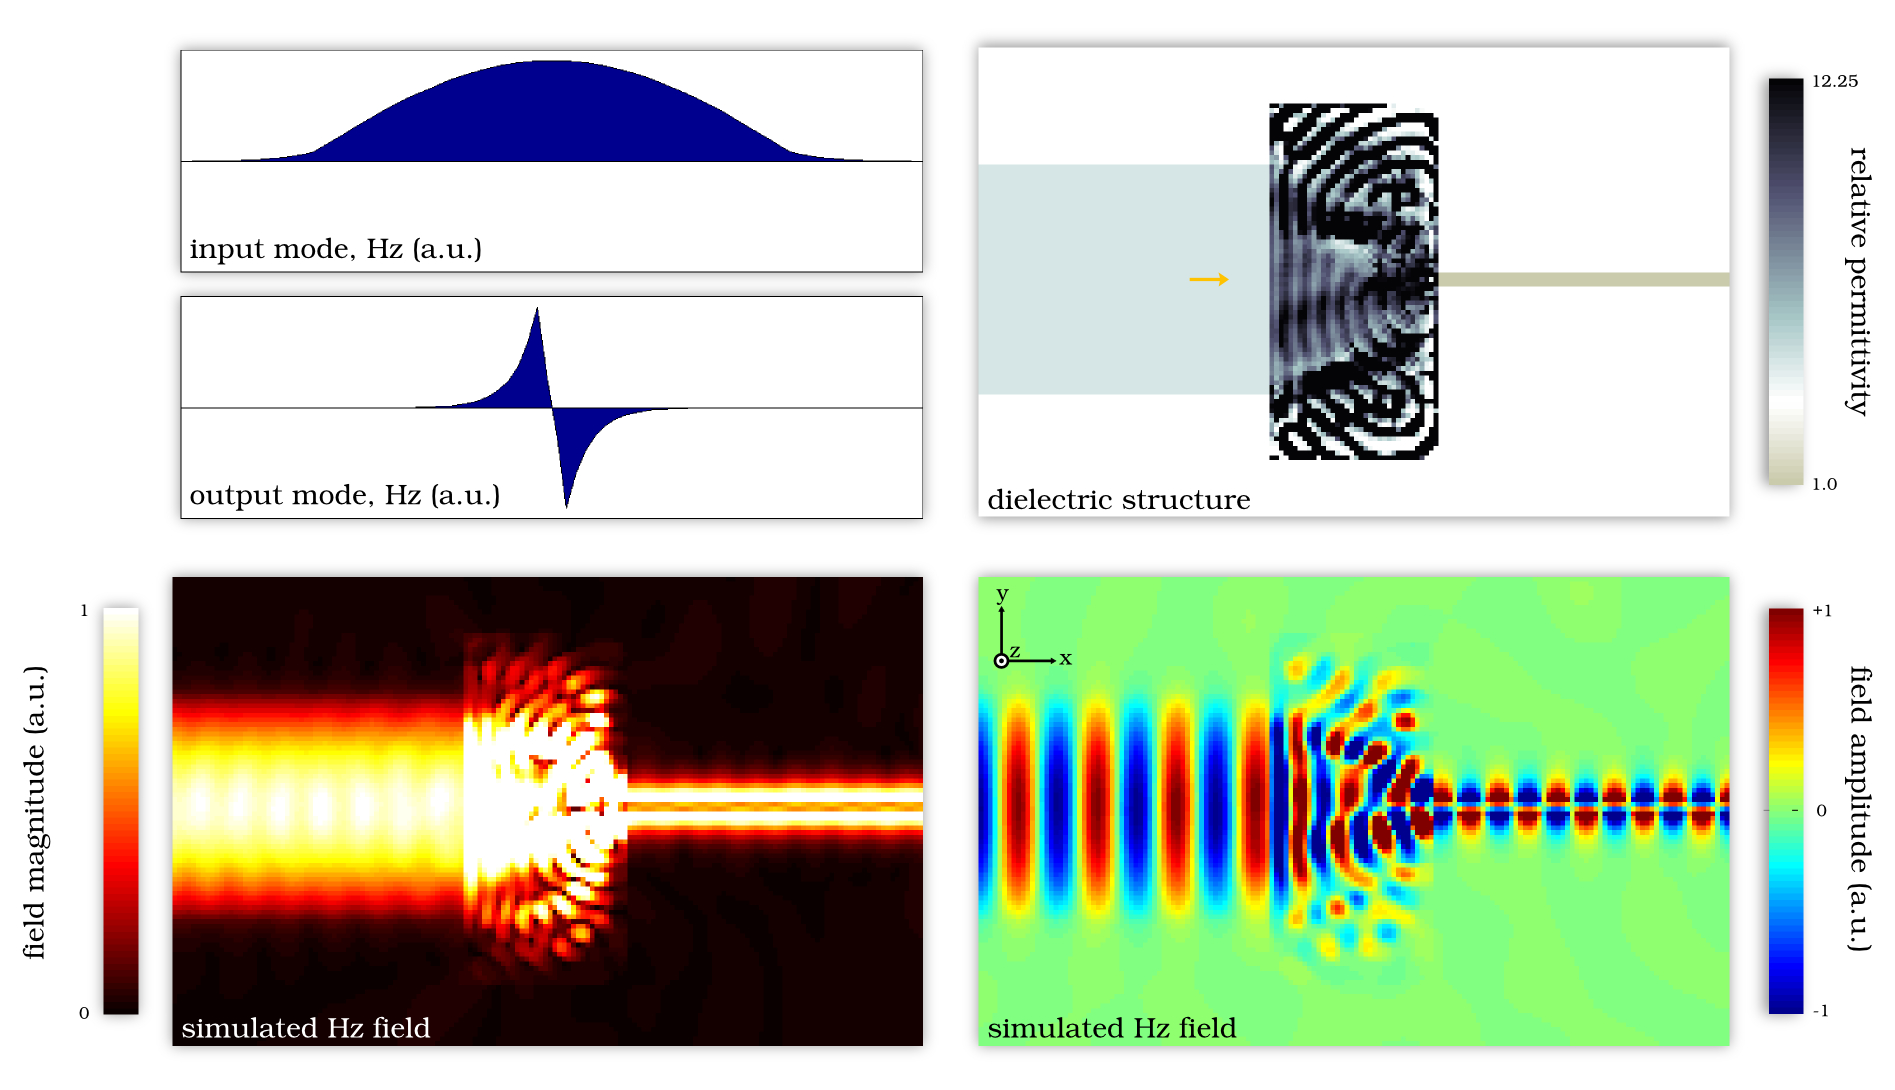
\includegraphics[width=\textwidth]{p3/15}
    \caption{
        Coupler from a wide, low-index waveguide to a
            plasmonic wire waveguide mode.
        Efficiency: $99.7\%$,
        footprint: $4.38$ square vacuum wavelengths.
        }
        % \label{fig:wire}
\end{figure}
\clearpage

\section{Additional designs with multiple output plasmonic waveguides}
We also present ``selector'' designs where photons are coupled to 
    only one of five possible plasmonic output waveguides.
We demonstrate these selector designs for both metal-insulator-metal and
    metal-wire plasmonic waveguides.
\begin{figure}[h!]
    \centering
    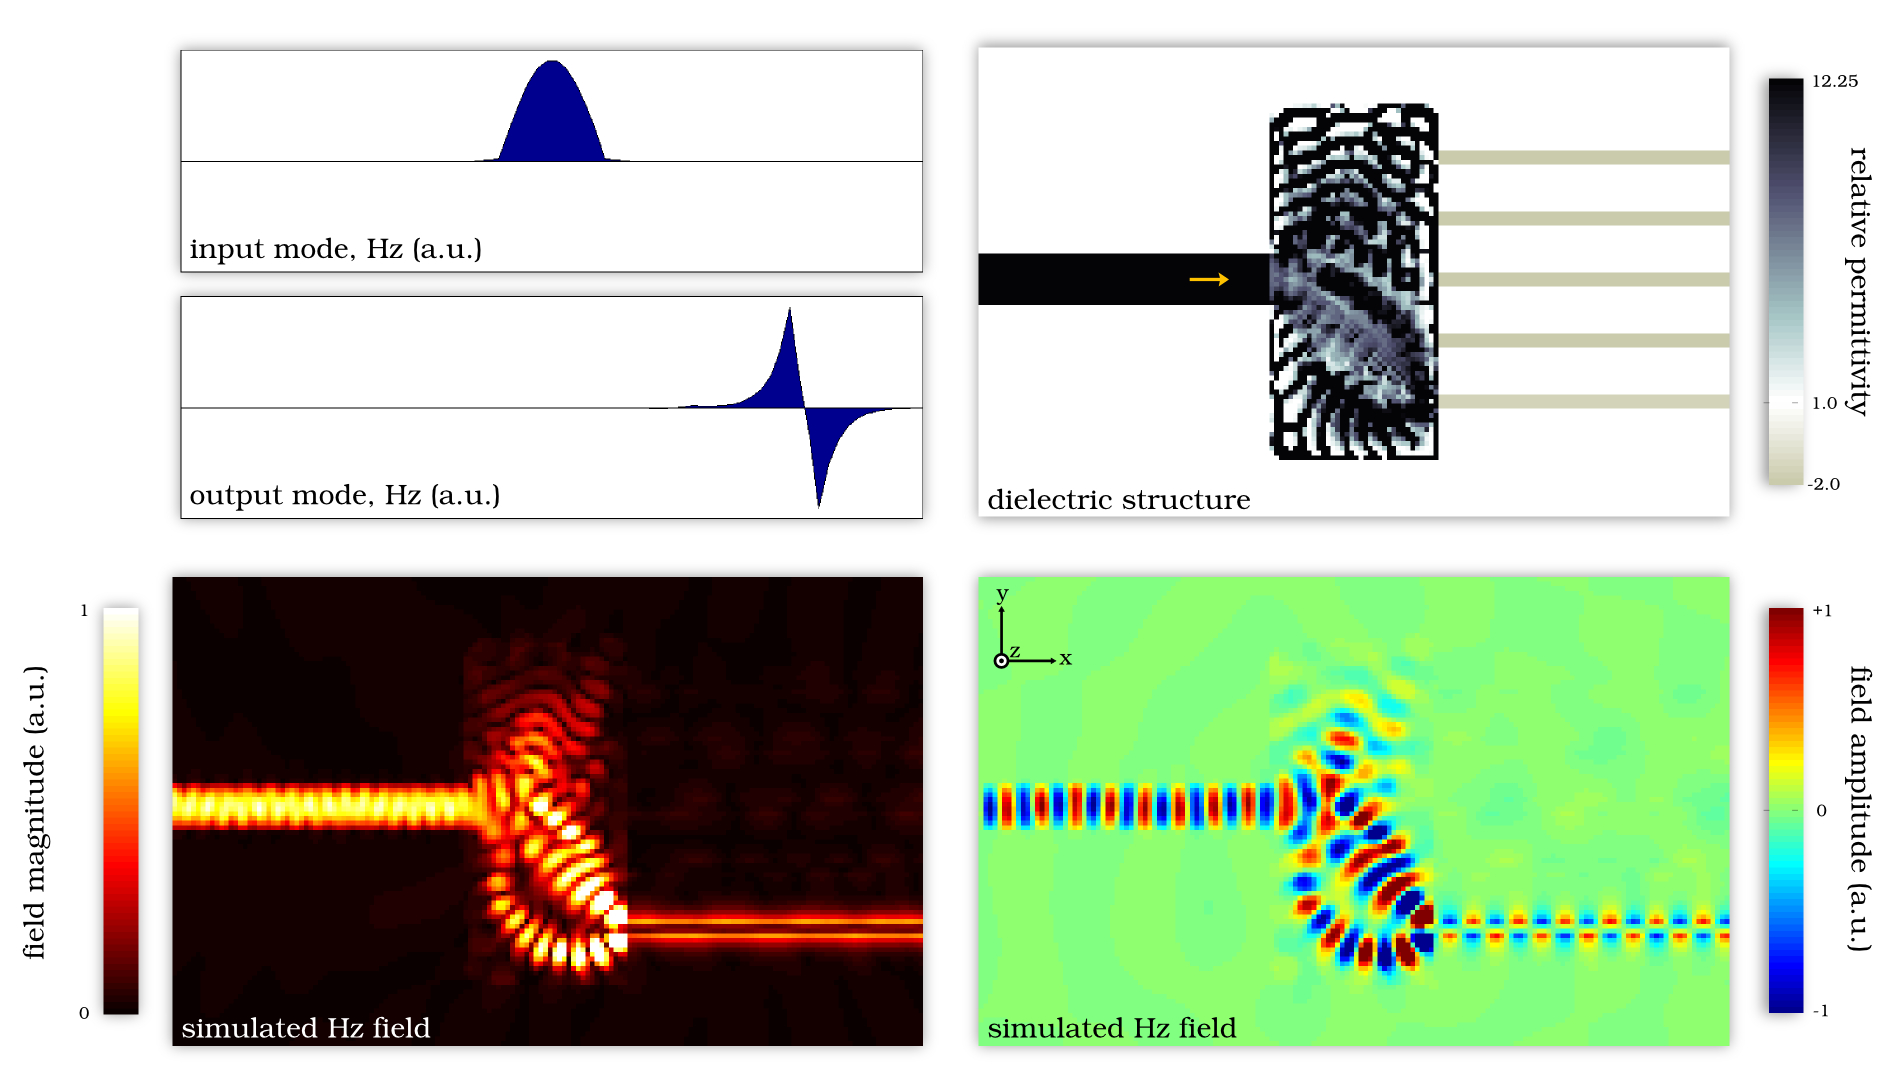
\includegraphics[width=\textwidth]{p3/16}
    \caption{
        Coupler from a dielectric waveguide to the 
            lowest branch of a set of five plasmonic wire waveguides.
        Efficiency: $94.0\%$,
        footprint: $4.38$ square vacuum wavelengths.
        }
        % \label{fig:wire}
\end{figure}
\begin{figure}[h!]
    \centering
    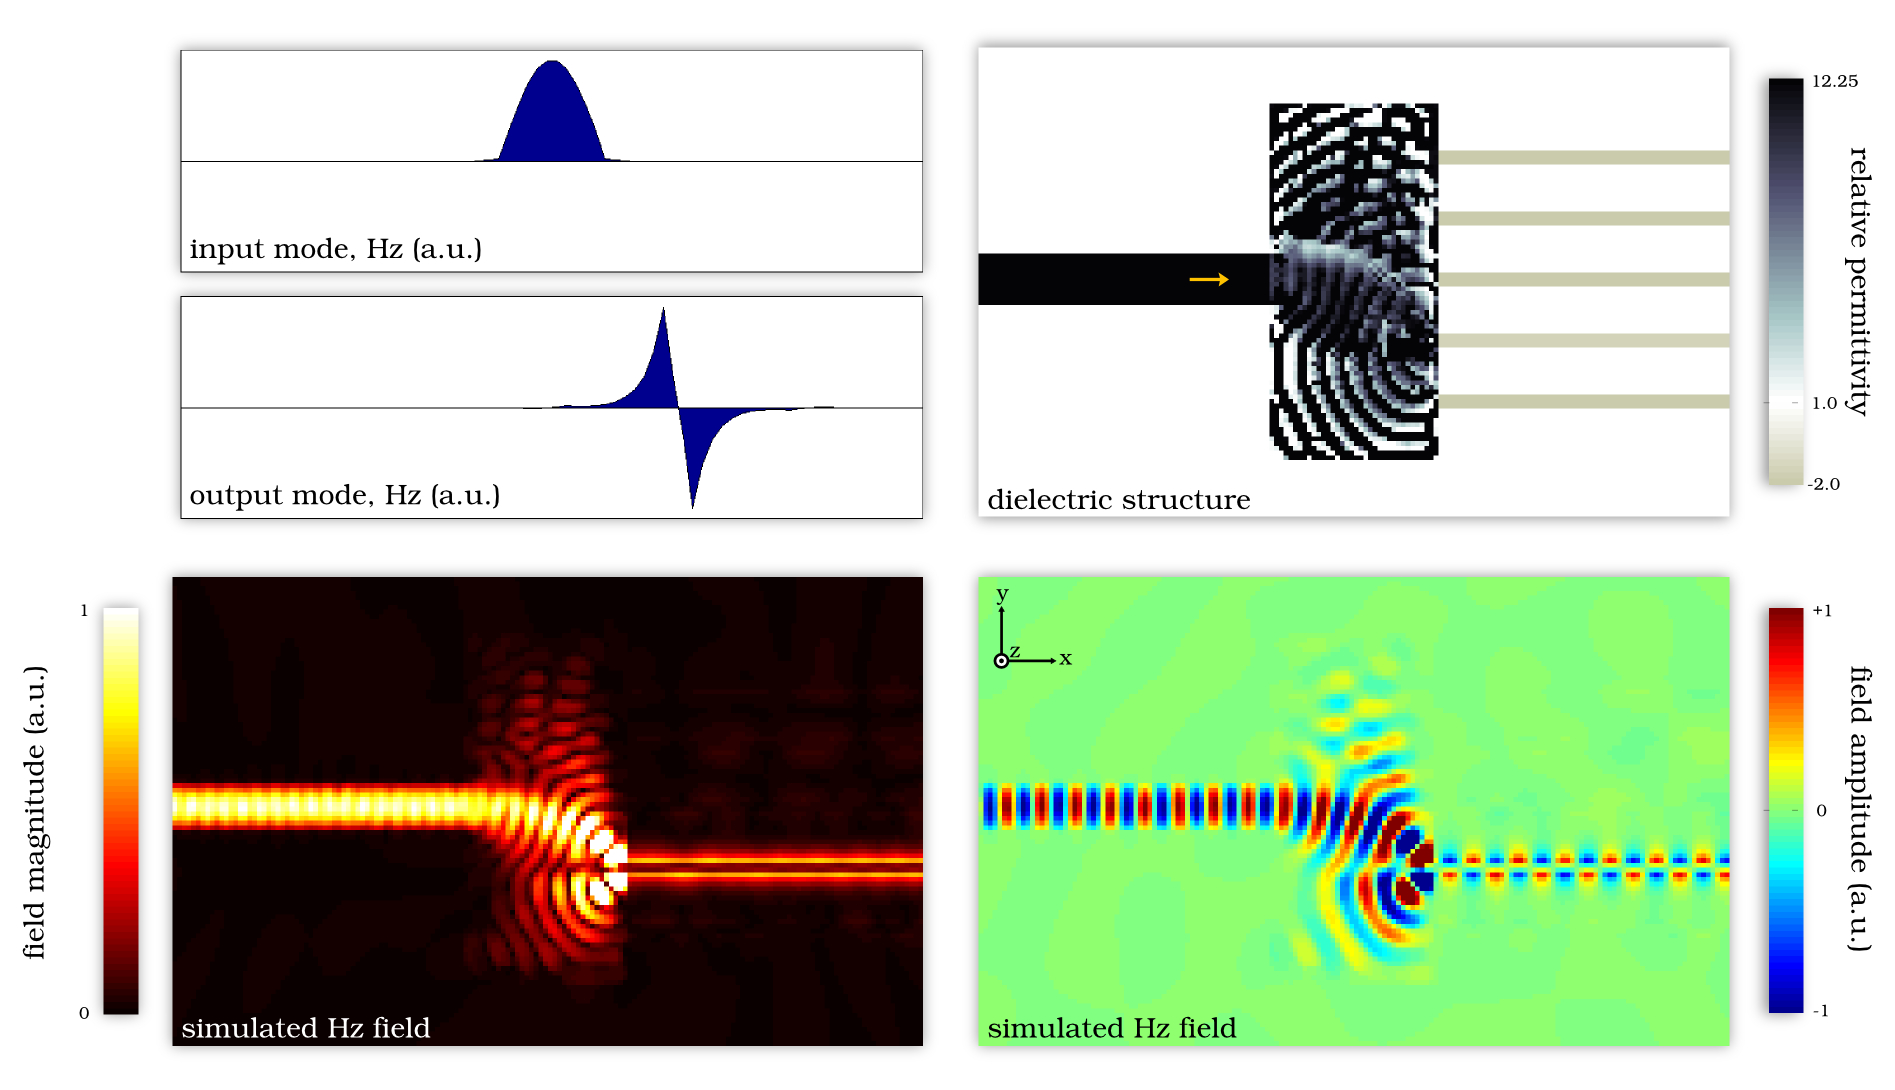
\includegraphics[width=\textwidth]{p3/17}
    \caption{
        Coupler from a dielectric waveguide to the 
            second branch of a set of five plasmonic wire waveguides.
        Efficiency: $97.3\%$,
        footprint: $4.38$ square vacuum wavelengths.
        }
        % \label{fig:wire}
\end{figure}
\begin{figure}[h!]
    \centering
    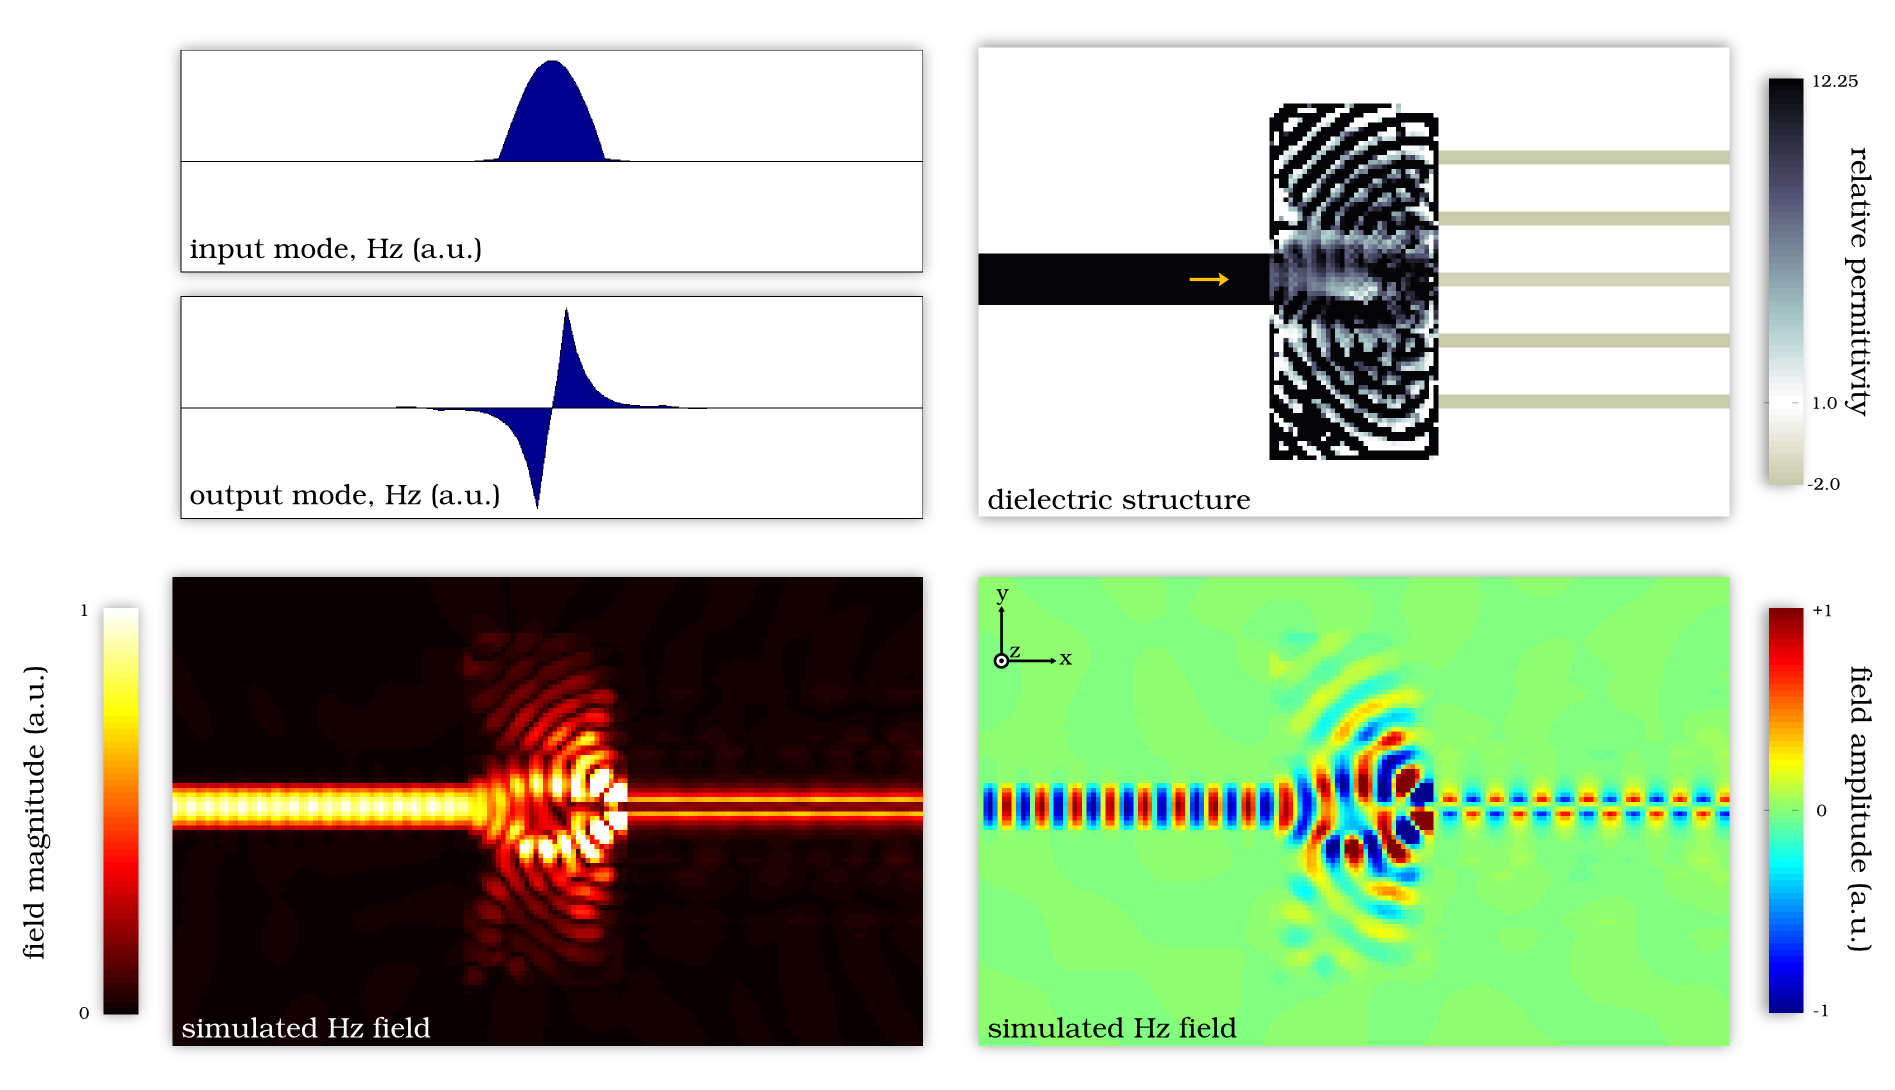
\includegraphics[width=\textwidth]{p3/18}
    \caption{
        Coupler from a dielectric waveguide to the 
            middle branch of a set of five plasmonic wire waveguides.
        Efficiency: $98.5\%$,
        footprint: $4.38$ square vacuum wavelengths.
        }
        % \label{fig:wire}
\end{figure}
\begin{figure}[h!]
    \centering
    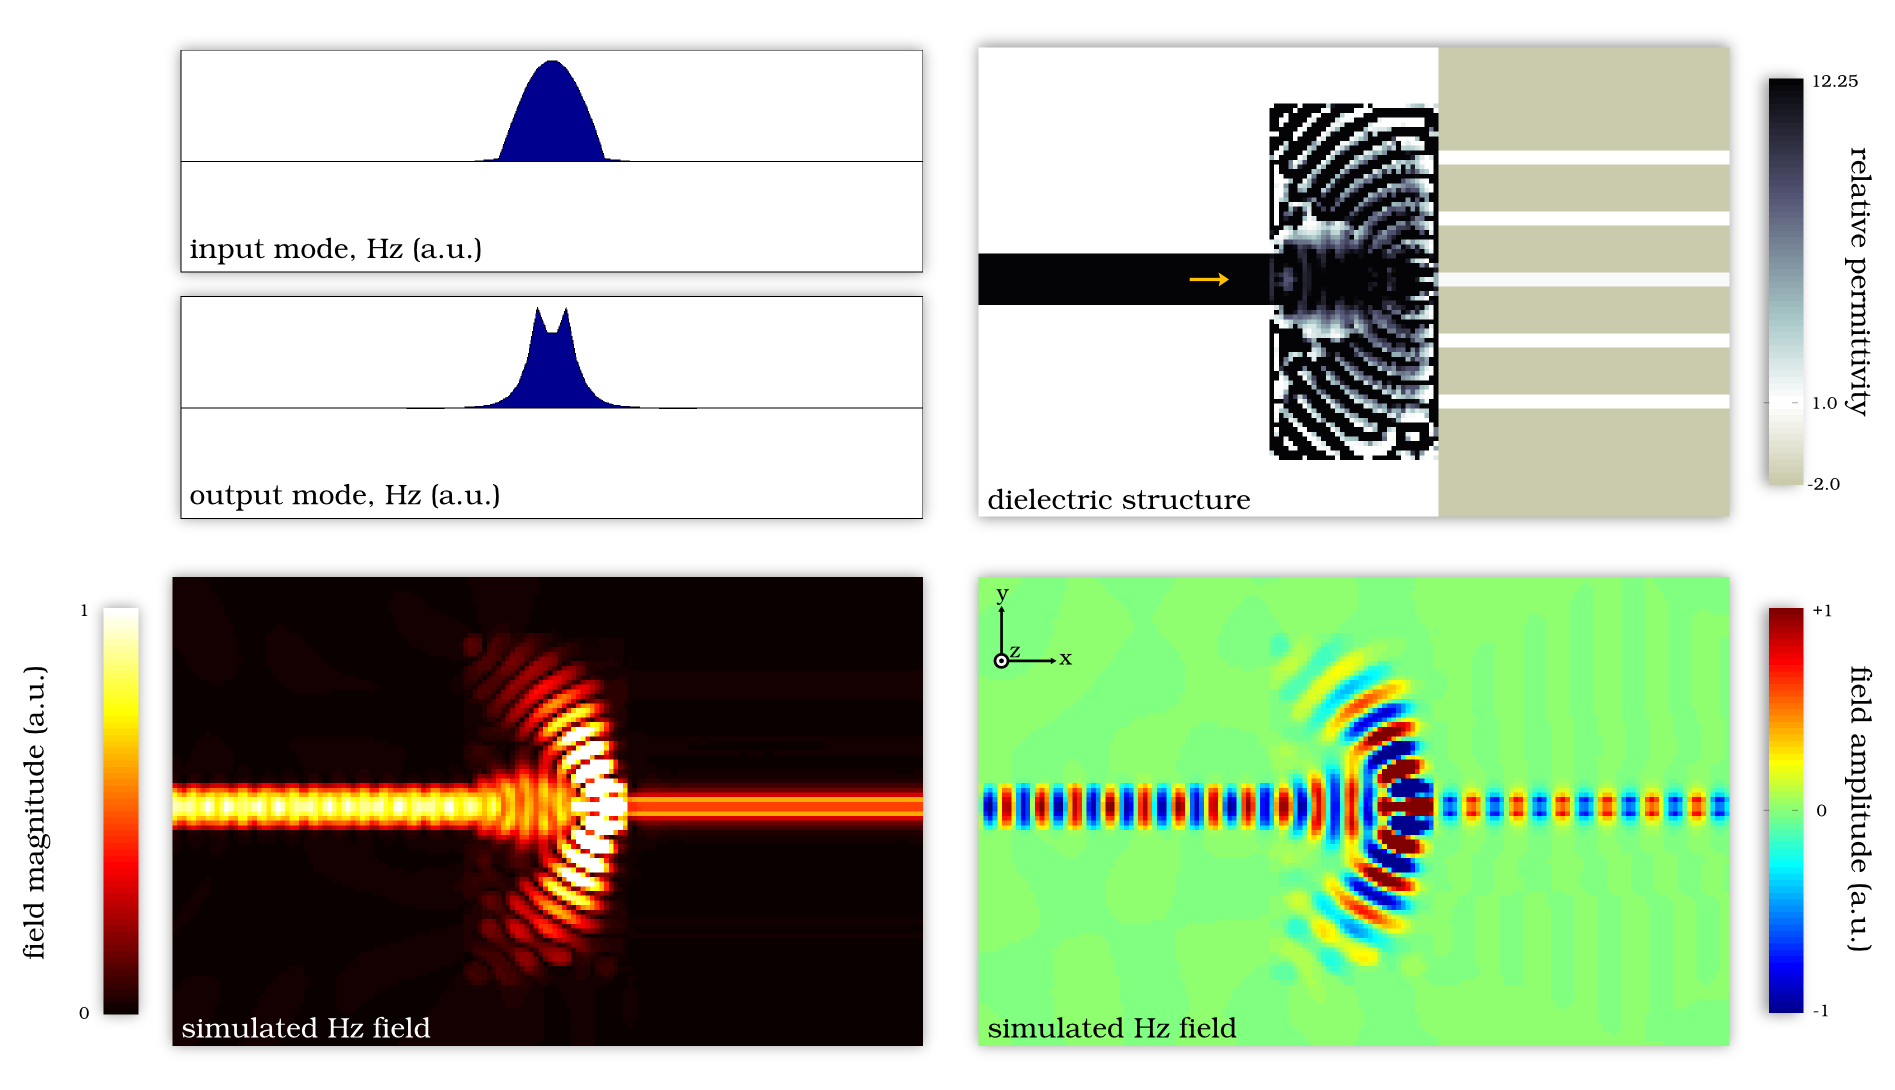
\includegraphics[width=\textwidth]{p3/19}
    \caption{
        Coupler from a dielectric waveguide to the 
            middle branch of a set of five plasmonic 
            metal-insulator-metal waveguides.
        Efficiency: $97.7\%$,
        footprint: $4.38$ square vacuum wavelengths.
        }
        % \label{fig:wire}
\end{figure}
\begin{figure}[h!]
    \centering
    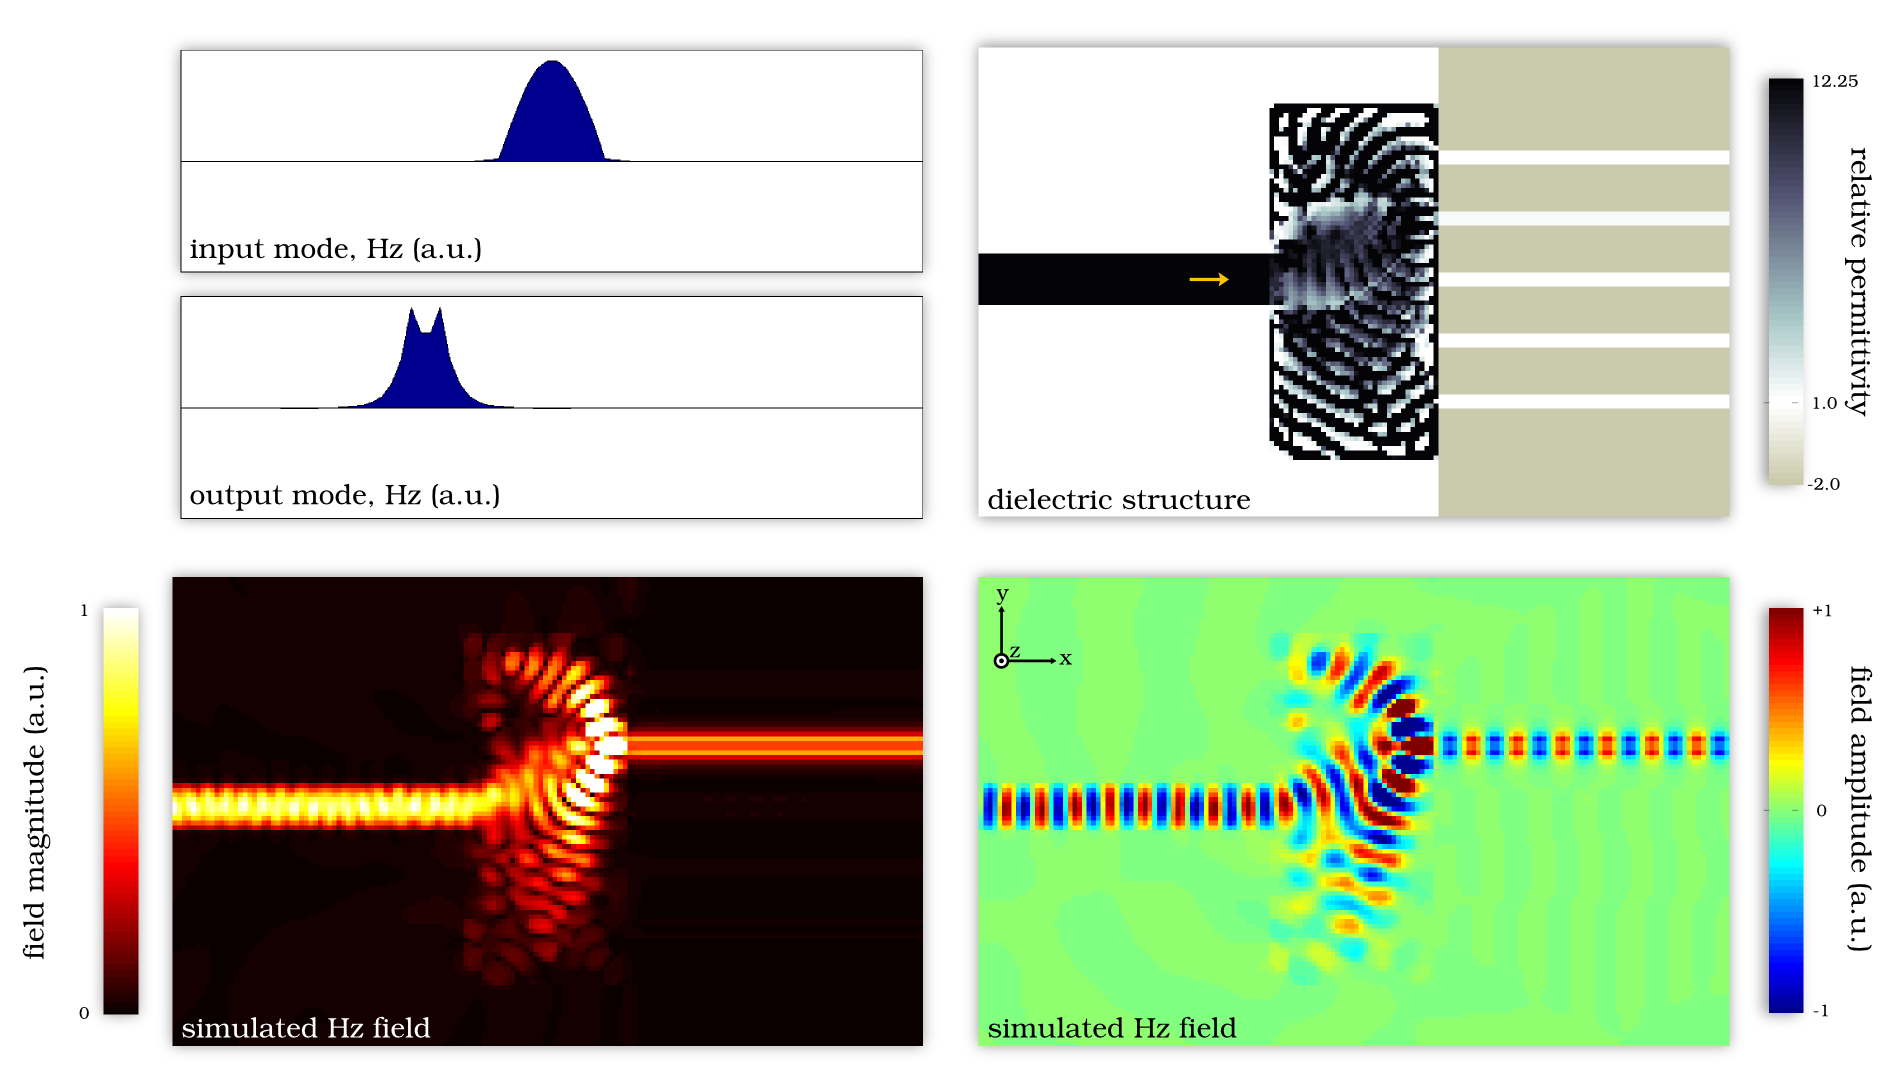
\includegraphics[width=\textwidth]{p3/20}
    \caption{
        Coupler from a dielectric waveguide to the 
            fourth branch of a set of five plasmonic 
            metal-insulator-metal waveguides.
        Efficiency: $95.6\%$,
        footprint: $4.38$ square vacuum wavelengths.
        }
        % \label{fig:wire}
\end{figure}
\begin{figure}[h!]
    \centering
    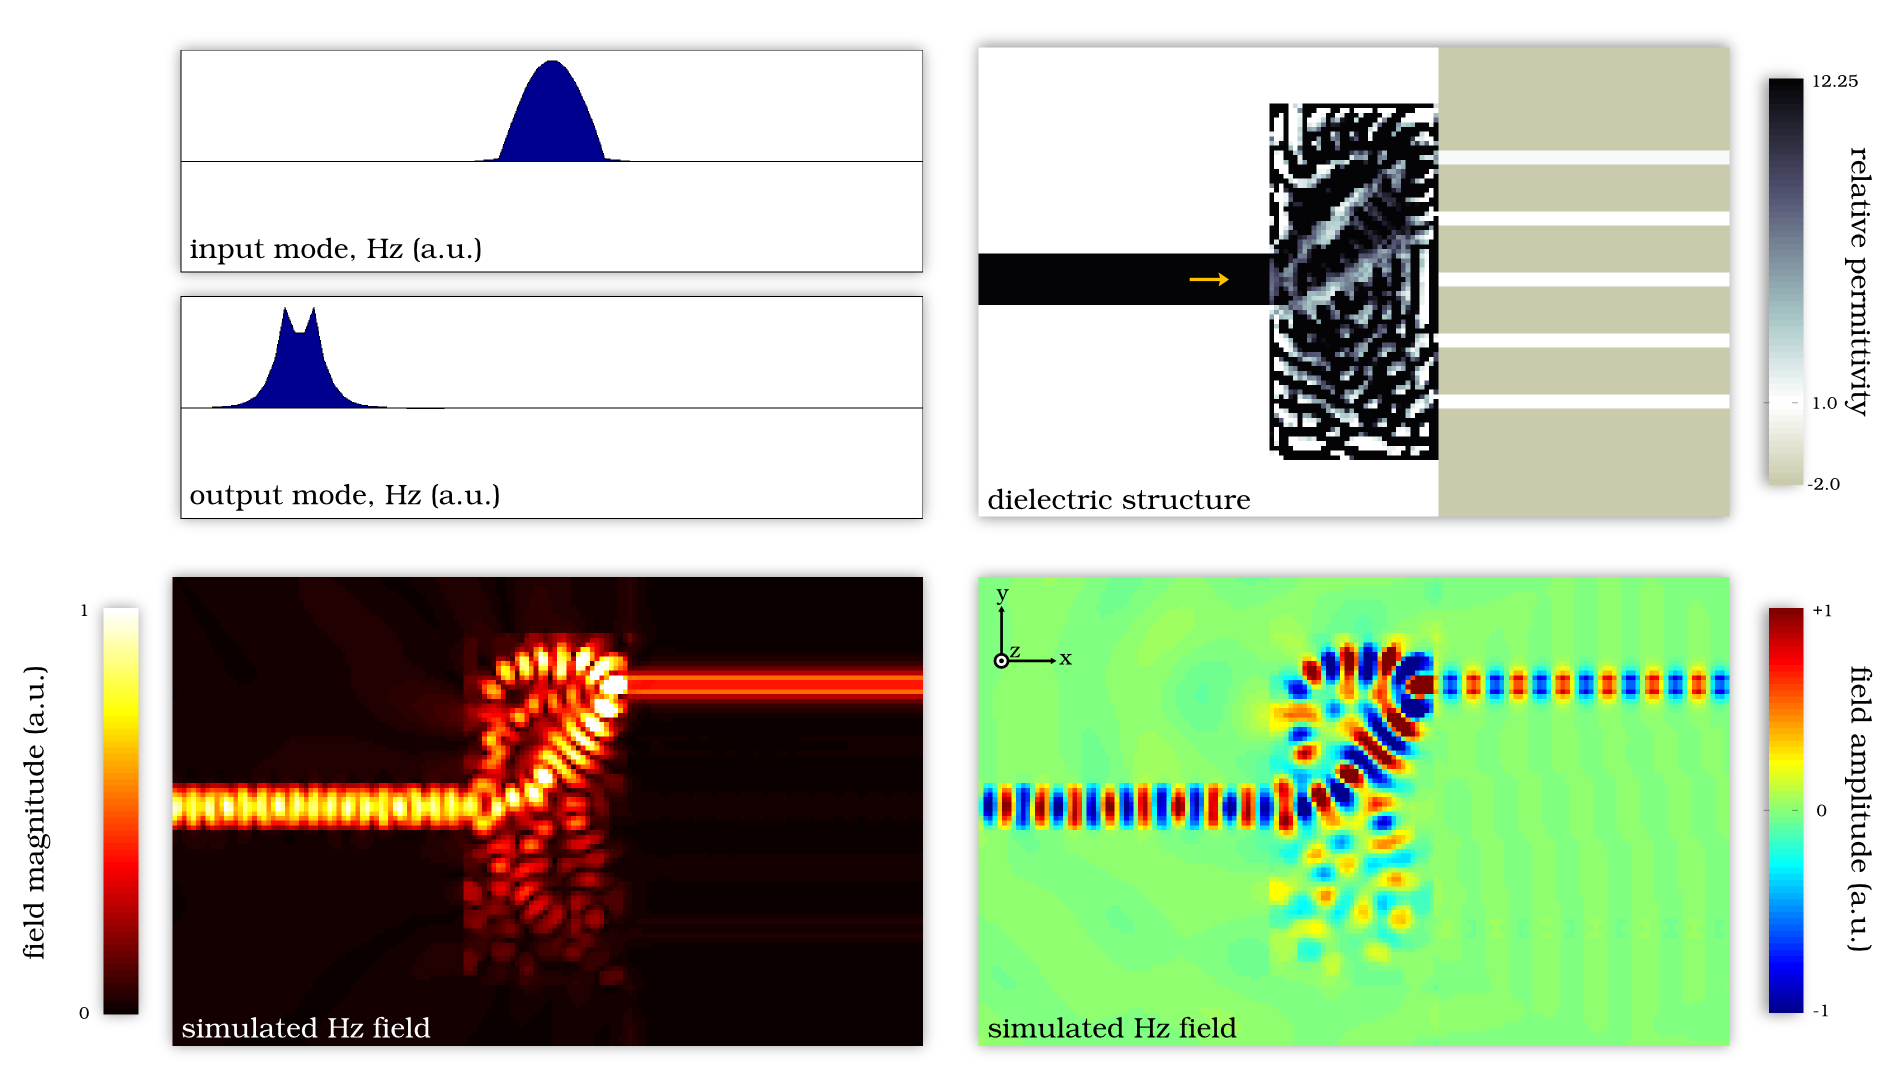
\includegraphics[width=\textwidth]{p3/21}
    \caption{
        Coupler from a dielectric waveguide to the 
            uppermost branch of a set of five plasmonic 
            metal-insulator-metal waveguides.
        Efficiency: $87.5\%$,
        footprint: $4.38$ square vacuum wavelengths.
        }
        % \label{fig:wire}
\end{figure}
\clearpage
% \end{appendix}

